
Before basis functions can be defined and PDEs can be discretised and solved 
we must first tesselate the domain with polygons, e.g. triangles and 
quadrilaterals in 2D, tetrahedra, prisms and hexahedra in 3D. \index{convex polygon} 

When the domain is itself simple (e.g. a rectangle, a sphere, ...) the mesh (or grid) can 
be (more or less) easily produced and the connectivity array filled with straightforward 
algorithms \cite{thie18}.
However, real life applications can involve etremely complex geometries (e.g. a bridge, 
a human spine, a car chassis and body, etc ...) and dedicated algorithms/softwares 
must be used (see \cite{thsw,frge,xiyz09}). 

We usually distinguish between two broad classes of grids: structured grids (with a regular 
connectivity) and unstructured grids (with an irregular connectivity).
\index{structured grid} \index{unstructured grid}

\begin{center}
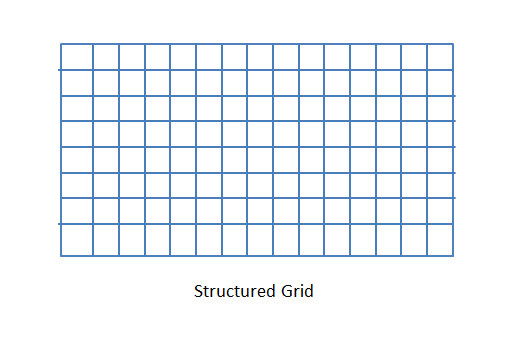
\includegraphics[width=5cm]{images/meshes/structured_grid}
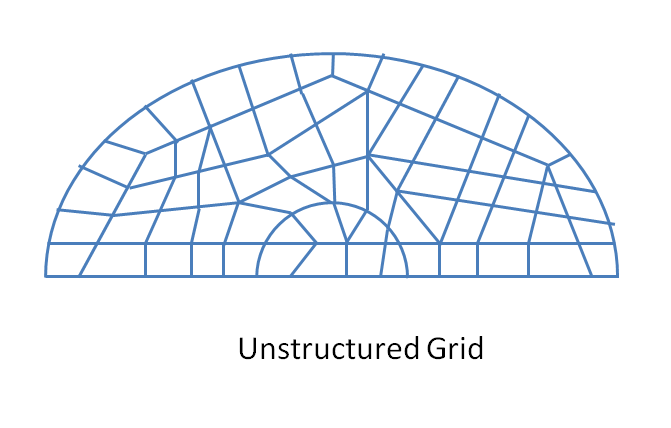
\includegraphics[width=5cm]{images/meshes/unstructured_grid}
\end{center}

On the following figure are shown various triangle- tetrahedron-based meshes. 
These are obviously better suited for simulations of complex geometries:
\begin{center}
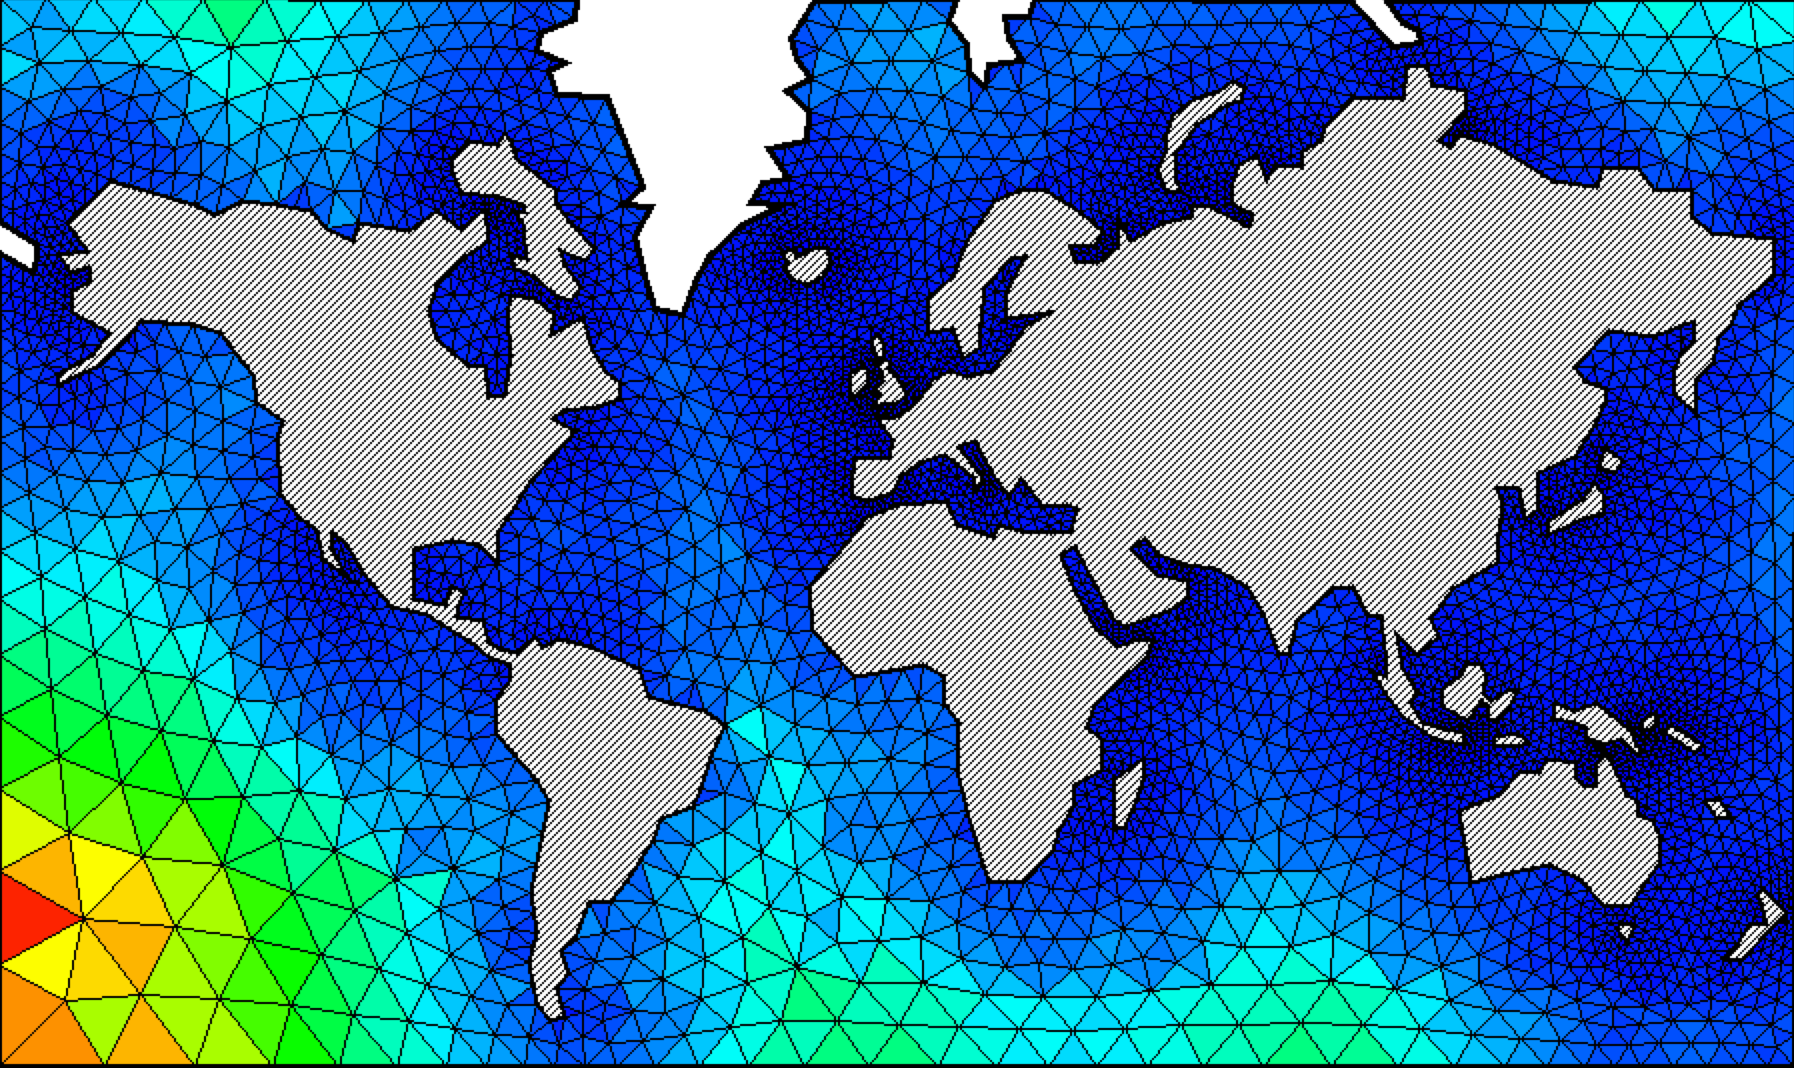
\includegraphics[height=4cm]{images/meshes/tr1.png}
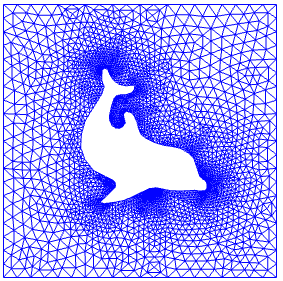
\includegraphics[height=4cm]{images/meshes/dolfin.png}
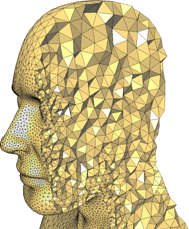
\includegraphics[height=4cm]{images/meshes/tetra.png}\\
\end{center}
\improvement[inline]{add more examples coming from geo}

Let us now focus on the case of a rectangular computational domain of size 
{\tt Lx} $\times$ {\tt Ly} with a regular mesh composed of {\tt nelx}$\times${\tt nely}={\tt nel}
   quadrilaterals.  
There are then {\tt nnx}$\times${\tt nny}={\tt nnp} grid points.
The elements are of size {\tt hx}$\times${\tt hy} with {\tt hx}={\tt Lx}/{\tt nelx}.

We have no reason to come up with an irregular/ilogical node numbering so 
we can number nodes row by row or column by column as shown on the example 
hereunder of a 3$\times$2 grid:

\begin{verbatim}
8=======9======10======11       2=======5=======8======11
|       |       |       |       |       |       |       |
|  (3)  |  (4)  |  (5)  |       |  (1)  |  (3)  |  (5)  |
|       |       |       |       |       |       |       |
4=======5=======6=======7       1=======4=======7======10
|       |       |       |       |       |       |       |
|  (0)  |  (1)  |  (2)  |       |  (0)  |  (2)  |  (4)  |
|       |       |       |       |       |       |       |
0=======1=======2=======3       0=======3=======6=======9

     "row by row"                  "column by column"
\end{verbatim}

The numbering of the elements themselves could be done in a somewhat chaotic 
way but we follow the numbering of the nodes for simplicity.
The row by row option is the adopted one in \fieldstone and the coordinates of the 
points are computed as follows:

\begin{lstlisting}
x = np.empty(nnp, dtype=np.float64)
y = np.empty(nnp, dtype=np.float64)
counter = 0
for j in range(0,nny):
    for i in range(0,nnx):
        x[counter]=i*hx
        y[counter]=j*hy
        counter += 1
\end{lstlisting}
The inner loop has {\tt i} ranging from {\tt 0} to {\tt nnx-1} first for {\tt j}=0, 1, ...
up to {\tt nny-1} which indeed corresponds to the row by row numbering.

\index{connectivity array} 
We now turn to the connectivity. As mentioned before, this is a structured mesh so that the so-called
connectivity array, named {\tt icon} in our case, can be filled easily. For each element we need
to store the node identities of its vertices. Since there are {\tt nel} elements and {\tt m=4} corners, 
this is a {\tt m}$\times${\tt nel} array. The algorithm goes as follows:

\begin{lstlisting}
icon =np.zeros((m,nel),dtype=np.int16)
counter = 0
for j in range(0,nely):
    for i in range(0,nelx):
        icon[0,counter] = i + j * nnx 
        icon[1,counter] = i + 1 + j * nnx 
        icon[2,counter] = i + 1 + (j + 1) * nnx 
        icon[3,counter] = i + (j + 1) * nnx 
        counter += 1
\end{lstlisting}

In the case of the 3$\times$2 mesh, the {\tt icon} is filled as follows:
\begin{center}
\begin{tabular}{ccccccc}
element id$\rightarrow$ &0 &1&2&3&4&5 \\
node id$\downarrow$ \\
0& 0& 1& 2& 4& 5  &6\\
1& 1& 2& 3& 5& 6  &7\\
2& 5& 6& 7& 9& 10 &11\\
3& 4& 5& 6& 8& 9  &10\\
\end{tabular}
\end{center}
It is to be understood as follows: element $\#4$ is composed of nodes 5, 6, 10 and 9.
Note that nodes are always stored in a counter clockwise manner, starting at the bottom left.
This is very important since the corresponding basis functions and their derivatives 
will be labelled accordingly.

In three dimensions things are very similar. The mesh now counts 
{\tt nelx}$\times${\tt nely}$\times${\tt nelz}={\tt nel} elements which represent 
a cuboid of size {\tt Lx}$\times${\tt Ly}$\times${\tt Lz}.
The position of the nodes is obtained as follows:
\begin{lstlisting}
x = np.empty(nnp,dtype=np.float64)
y = np.empty(nnp,dtype=np.float64)
z = np.empty(nnp,dtype=np.float64)
counter=0
for i in range(0,nnx):
    for j in range(0,nny):
        for k in range(0,nnz):
            x[counter]=i*hx
            y[counter]=j*hy
            z[counter]=k*hz
            counter += 1
\end{lstlisting}
The connectivity array is now of size {\tt m}$\times${\tt nel} with {\tt m=8}:
\begin{lstlisting}
icon =np.zeros((m,nel),dtype=np.int16)
counter = 0
for i in range(0,nelx):
    for j in range(0,nely):
        for k in range(0,nelz):
            icon[0,counter]=nny*nnz*(i  )+nnz*(j  )+k
            icon[1,counter]=nny*nnz*(i+1)+nnz*(j  )+k
            icon[2,counter]=nny*nnz*(i+1)+nnz*(j+1)+k
            icon[3,counter]=nny*nnz*(i  )+nnz*(j+1)+k
            icon[4,counter]=nny*nnz*(i  )+nnz*(j  )+k+1
            icon[5,counter]=nny*nnz*(i+1)+nnz*(j  )+k+1
            icon[6,counter]=nny*nnz*(i+1)+nnz*(j+1)+k+1
            icon[7,counter]=nny*nnz*(i  )+nnz*(j+1)+k+1
            counter += 1
\end{lstlisting}

\improvement[inline]{produce drawing of node numbering}



